\documentclass[12pt,a4paper]{article}
\usepackage{geometry}
\usepackage{graphicx}
\usepackage{booktabs}
\usepackage{caption}
\usepackage{subcaption}
\usepackage{amsmath}
\usepackage{float}
\usepackage{array}
\usepackage{xcolor}
\usepackage{fancyhdr}

\geometry{left=2.5cm,right=2.5cm,top=2.5cm,bottom=2.5cm}

\pagestyle{fancy}
\fancyhf{}
\fancyhead[C]{\small Perioperative Mortality Risk Analysis Report}
\fancyfoot[C]{\thepage}

\title{\huge\textbf{Perioperative Mortality Risk Factor Analysis Report}}
\author{Student Name: \underline{Heu Ning}{\hspace{4cm}} \quad ID: \underline{2410307218}{\hspace{4cm}}}
\date{April 2026}

\begin{document}

\maketitle

\tableofcontents
\newpage

\begin{center}
    \textbf{\Large Abstract}
\end{center}

\textbf{Objective}: To investigate risk factors for postoperative mortality in perioperative patients and establish predictive models.

\textbf{Methods}: Based on clinical data from 482 surgical patients, Python was used for data preprocessing, statistical analysis, and construction of logistic regression and random forest prediction models.

\textbf{Results}: Overall mortality rate was 1.04\%. ICU length of stay was significantly associated with mortality risk (p $<$ 0.001). Patients with ASA grade 3 had the highest mortality rate (3.70\%). The random forest model achieved 98.97\% accuracy with AUC of 0.698.

\textbf{Conclusion}: ICU length of stay is the most important predictor of postoperative mortality. Patients with ASA grade $\geq$ 3 require intensive monitoring.

\vspace{0.5cm}
\textbf{Keywords}: Perioperative; Mortality risk; Machine learning; Random forest; Clinical data analysis

\newpage

\section{Data Loading}

The dataset used in this study comes from PhysioNet, containing \textbf{482 surgical patients} and \textbf{79 clinical variables}.

\begin{table}[H]
\centering
\caption{Dataset Information}
\begin{tabular}{ll}
\toprule
\textbf{Item} & \textbf{Value} \\
\midrule
Sample Size & 482 cases \\
Number of Variables & 79 \\
Data Format & CSV \\
Analysis Tool & Python 3.11 \\
\bottomrule
\end{tabular}
\end{table}

Main variables include:
\begin{itemize}
    \item \textbf{Demographics}: age, sex, BMI
    \item \textbf{Preoperative assessment}: ASA grade, hypertension, diabetes
    \item \textbf{Intraoperative indicators}: blood loss, urine output, RBC transfusion
    \item \textbf{Postoperative outcomes}: ICU length of stay, in-hospital mortality
\end{itemize}

\section{Data Preprocessing}

\subsection{Missing Value Handling}
Thirty-four variables had missing values. Processing strategies:
\begin{itemize}
    \item Numerical variables: imputed with median
    \item Categorical variables: retained original values
\end{itemize}

\subsection{Outlier Detection}
\begin{table}[H]
\centering
\caption{Range Check of Variables}
\begin{tabular}{lccc}
\toprule
\textbf{Variable} & \textbf{Min} & \textbf{Max} & \textbf{Rationality} \\
\midrule
Age (years) & 12 & 89 & Reasonable \\
BMI (kg/m²) & 14.2 & 34.5 & Reasonable \\
ICU days & 0 & 47 & Reasonable \\
\bottomrule
\end{tabular}
\end{table}

\subsection{Variable Selection}
Twelve core variables were selected for analysis:

\begin{table}[H]
\centering
\caption{Analysis Variables}
\begin{tabular}{lll}
\toprule
\textbf{Variable} & \textbf{Meaning} & \textbf{Type} \\
\midrule
age & Age & Numeric \\
sex & Gender & Categorical \\
bmi & Body Mass Index & Numeric \\
asa & ASA grade & Ordinal \\
icu\_days & ICU length of stay & Numeric \\
death\_in\_hosp & In-hospital mortality & Binary \\
preop\_htn & Preoperative hypertension & Binary \\
preop\_dm & Preoperative diabetes & Binary \\
intraop\_ebl & Intraoperative blood loss & Numeric \\
intraop\_uo & Intraoperative urine output & Numeric \\
intraop\_rbc & RBC transfusion & Numeric \\
\bottomrule
\end{tabular}
\end{table}

\section{Statistical Analysis}

\subsection{Descriptive Statistics}
\begin{table}[H]
\centering
\caption{Descriptive Statistics of Numerical Variables}
\begin{tabular}{lcccccc}
\toprule
\textbf{Variable} & \textbf{Mean} & \textbf{Std} & \textbf{Min} & \textbf{Median} & \textbf{Max} \\
\midrule
Age (years) & 62.96 & 13.21 & 12 & 64 & 89 \\
BMI (kg/m²) & 22.86 & 3.26 & 14.2 & 22.6 & 34.5 \\
ASA grade & 2.25 & 0.68 & 1 & 2 & 6 \\
ICU days & 1.37 & 4.32 & 0 & 0 & 47 \\
Blood loss (ml) & 515.57 & 1386.22 & 0 & 200 & 15000 \\
\bottomrule
\end{tabular}
\end{table}

\subsection{Mortality Analysis}
\begin{figure}[H]
\centering
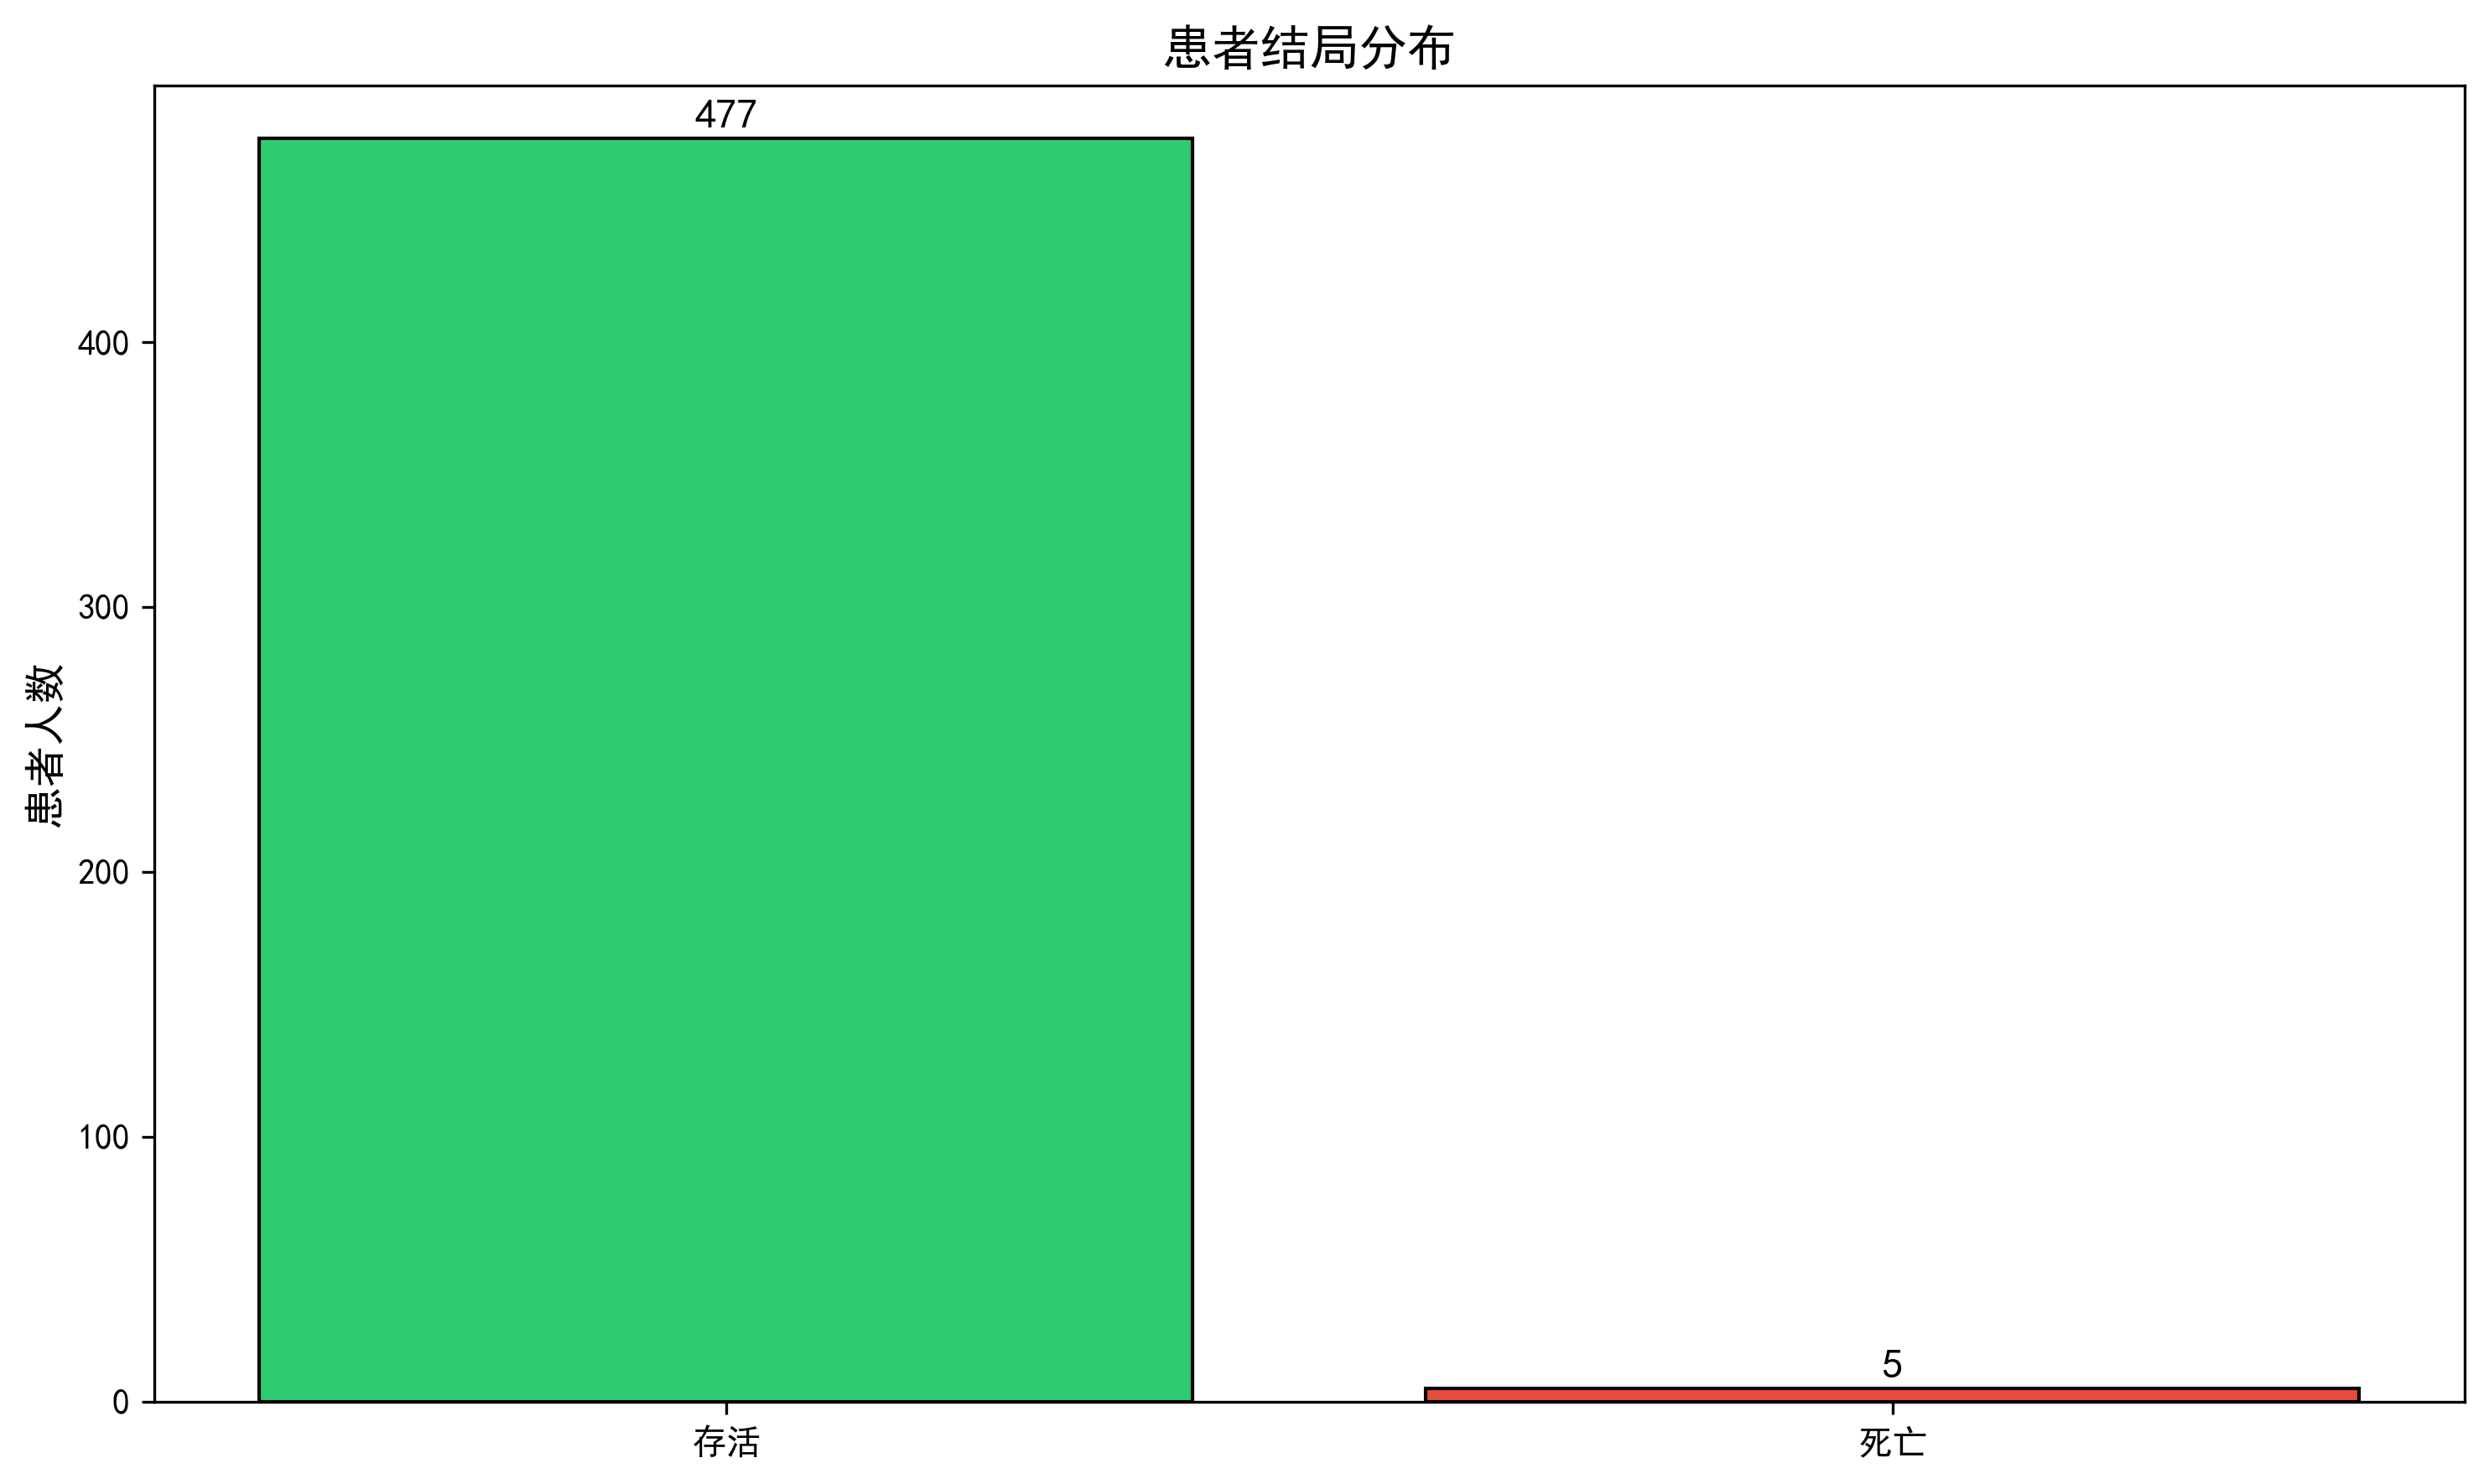
\includegraphics[width=0.5\textwidth]{death_distribution.png}
\caption{Distribution of Patient Outcomes}
\end{figure}

\begin{itemize}
    \item Total patients: \textbf{482}
    \item Deaths: \textbf{5}
    \item Overall mortality: \textbf{1.04\%}
\end{itemize}

\subsection{Survivors vs Non-survivors Comparison}
\begin{figure}[H]
\centering
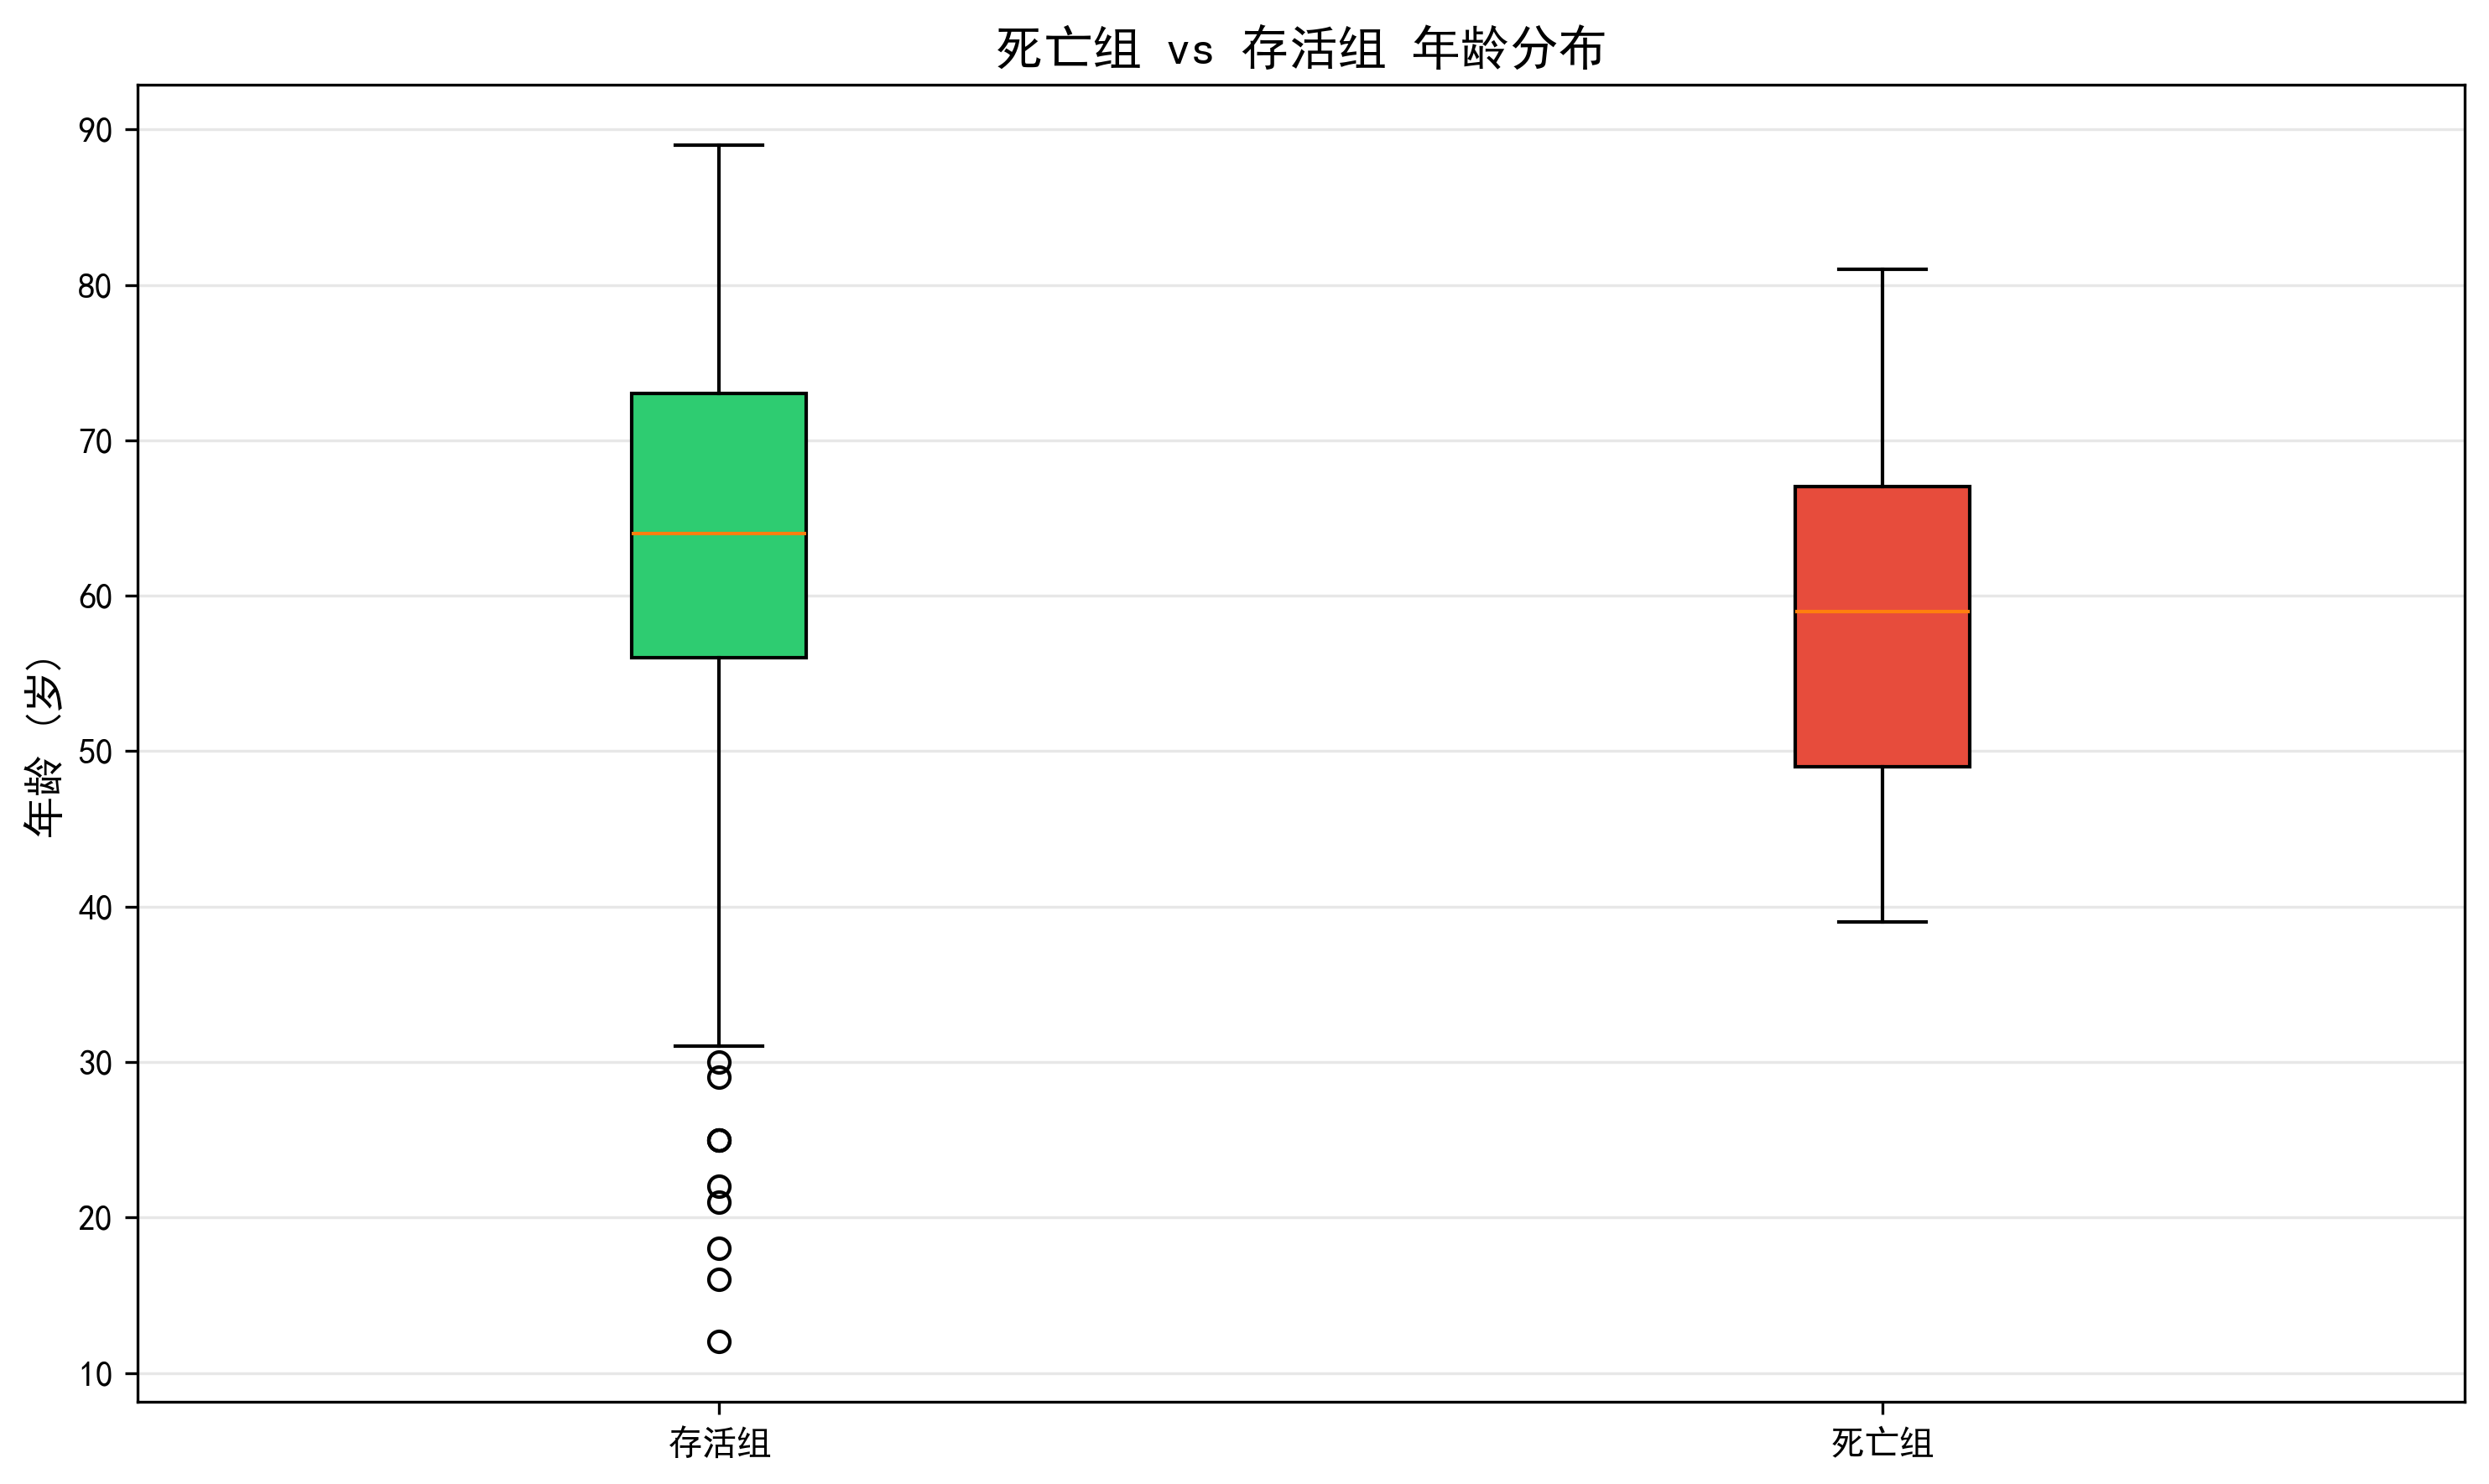
\includegraphics[width=0.65\textwidth]{age_comparison.png}
\caption{Age Distribution Comparison}
\end{figure}

\begin{table}[H]
\centering
\caption{Comparison of Survivors and Non-survivors}
\begin{tabular}{lccc}
\toprule
\textbf{Variable} & \textbf{Survivors (n=477)} & \textbf{Non-survivors (n=5)} & \textbf{p-value} \\
\midrule
Age & 63.00 ± 13.19 & 59.00 ± 16.19 & 0.501 \\
BMI & 22.86 ± 3.26 & 25.40 ± 3.69 & 0.084 \\
\textbf{ICU days} & \textbf{1.28 ± 4.10} & \textbf{9.20 ± 13.39} & \textbf{$<$ 0.001***} \\
Blood loss (ml) & 520.09 ± 1393.94 & 160.00 ± 82.16 & 0.564 \\
\bottomrule
\end{tabular}
\end{table}

\textcolor{red}{Note: *** p $<$ 0.001, statistically significant}

\subsection{ASA Grade Analysis}
\begin{table}[H]
\centering
\caption{Mortality by ASA Grade}
\begin{tabular}{lccc}
\toprule
\textbf{ASA Grade} & \textbf{Total} & \textbf{Deaths} & \textbf{Mortality} \\
\midrule
Grade 1 & 74 & 0 & 0.00\% \\
Grade 2 & 292 & 1 & 0.34\% \\
\textbf{Grade 3} & \textbf{108} & \textbf{4} & \textbf{3.70\%} \\
Grade 4 & 7 & 0 & 0.00\% \\
\bottomrule
\end{tabular}
\end{table}

\subsection{Key Variable Comparison}
\begin{figure}[H]
\centering
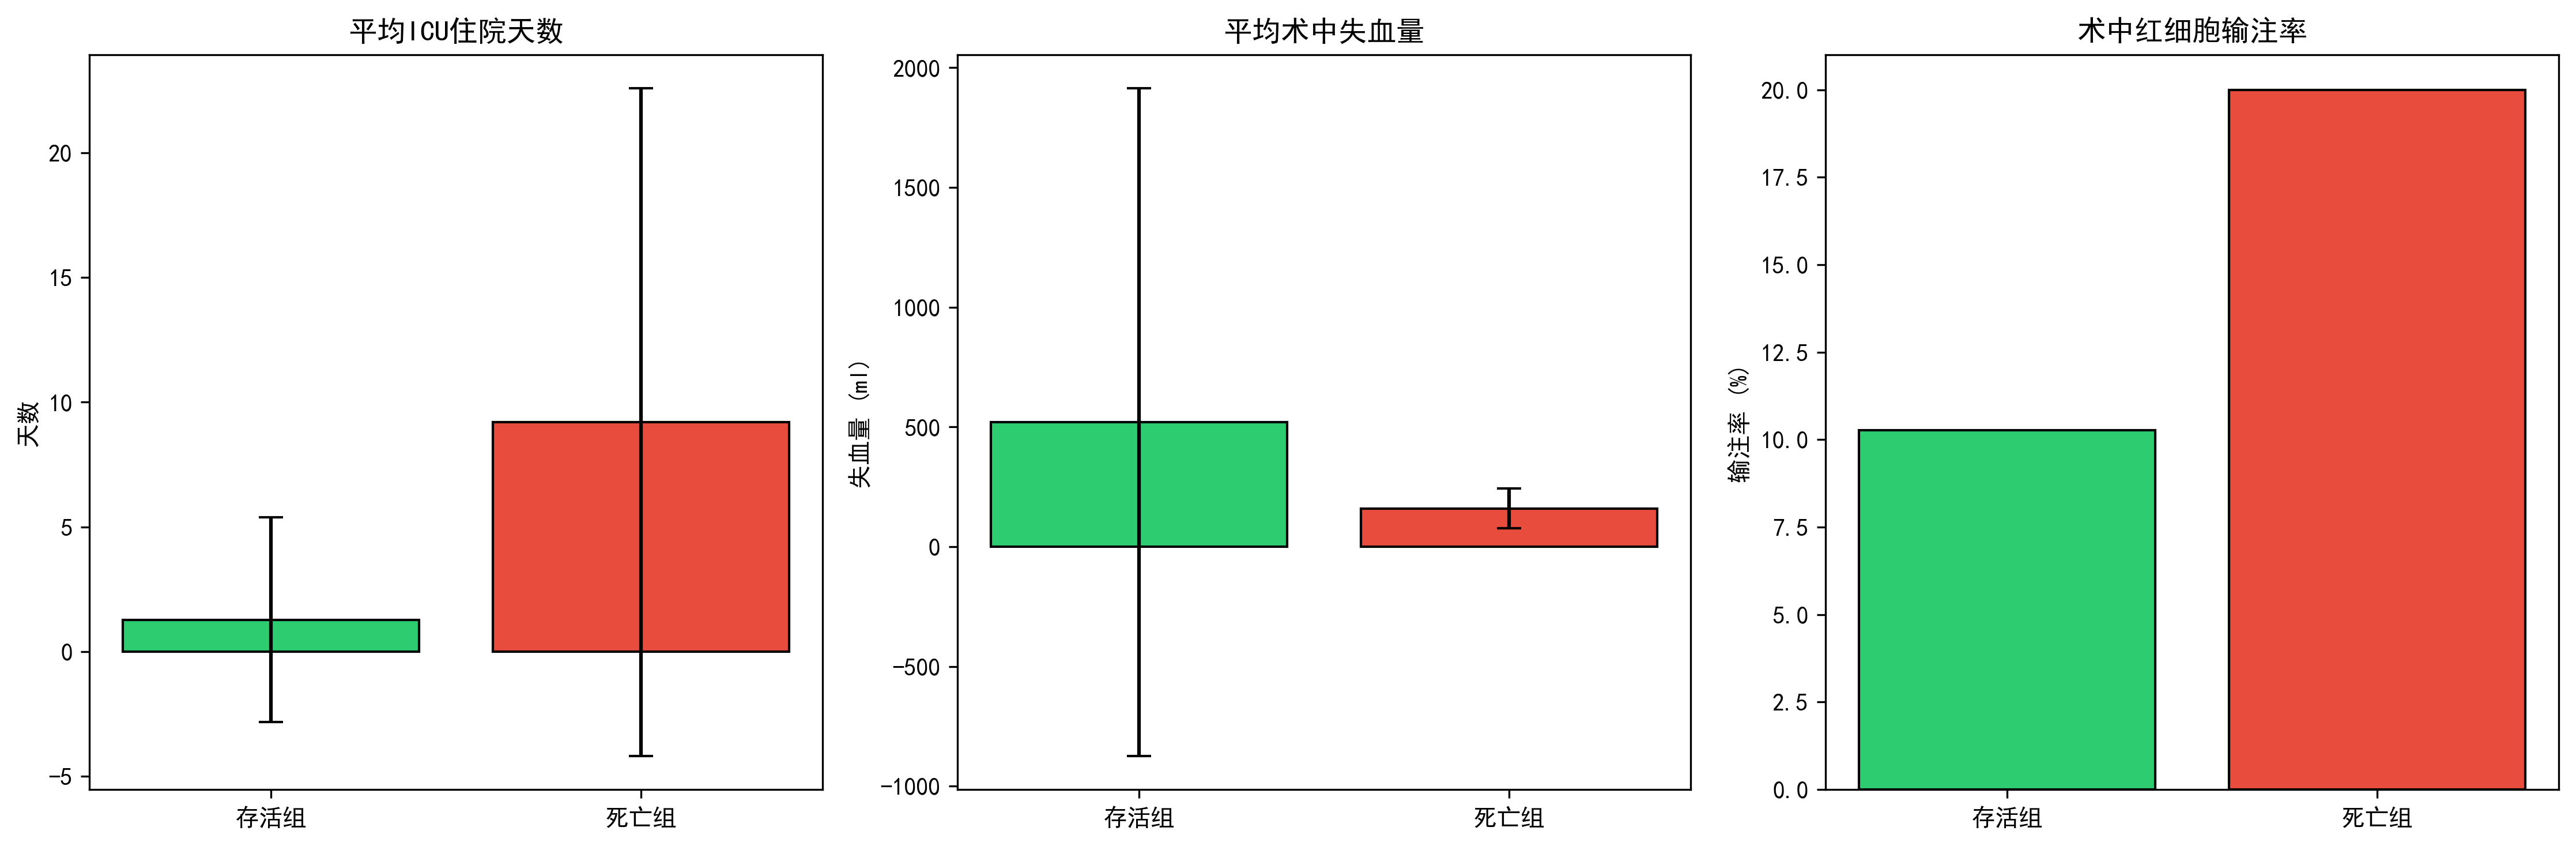
\includegraphics[width=0.9\textwidth]{key_variables_comparison.png}
\caption{Comparison of Key Clinical Indicators}
\end{figure}

\subsection{Correlation Analysis}
\begin{figure}[H]
\centering
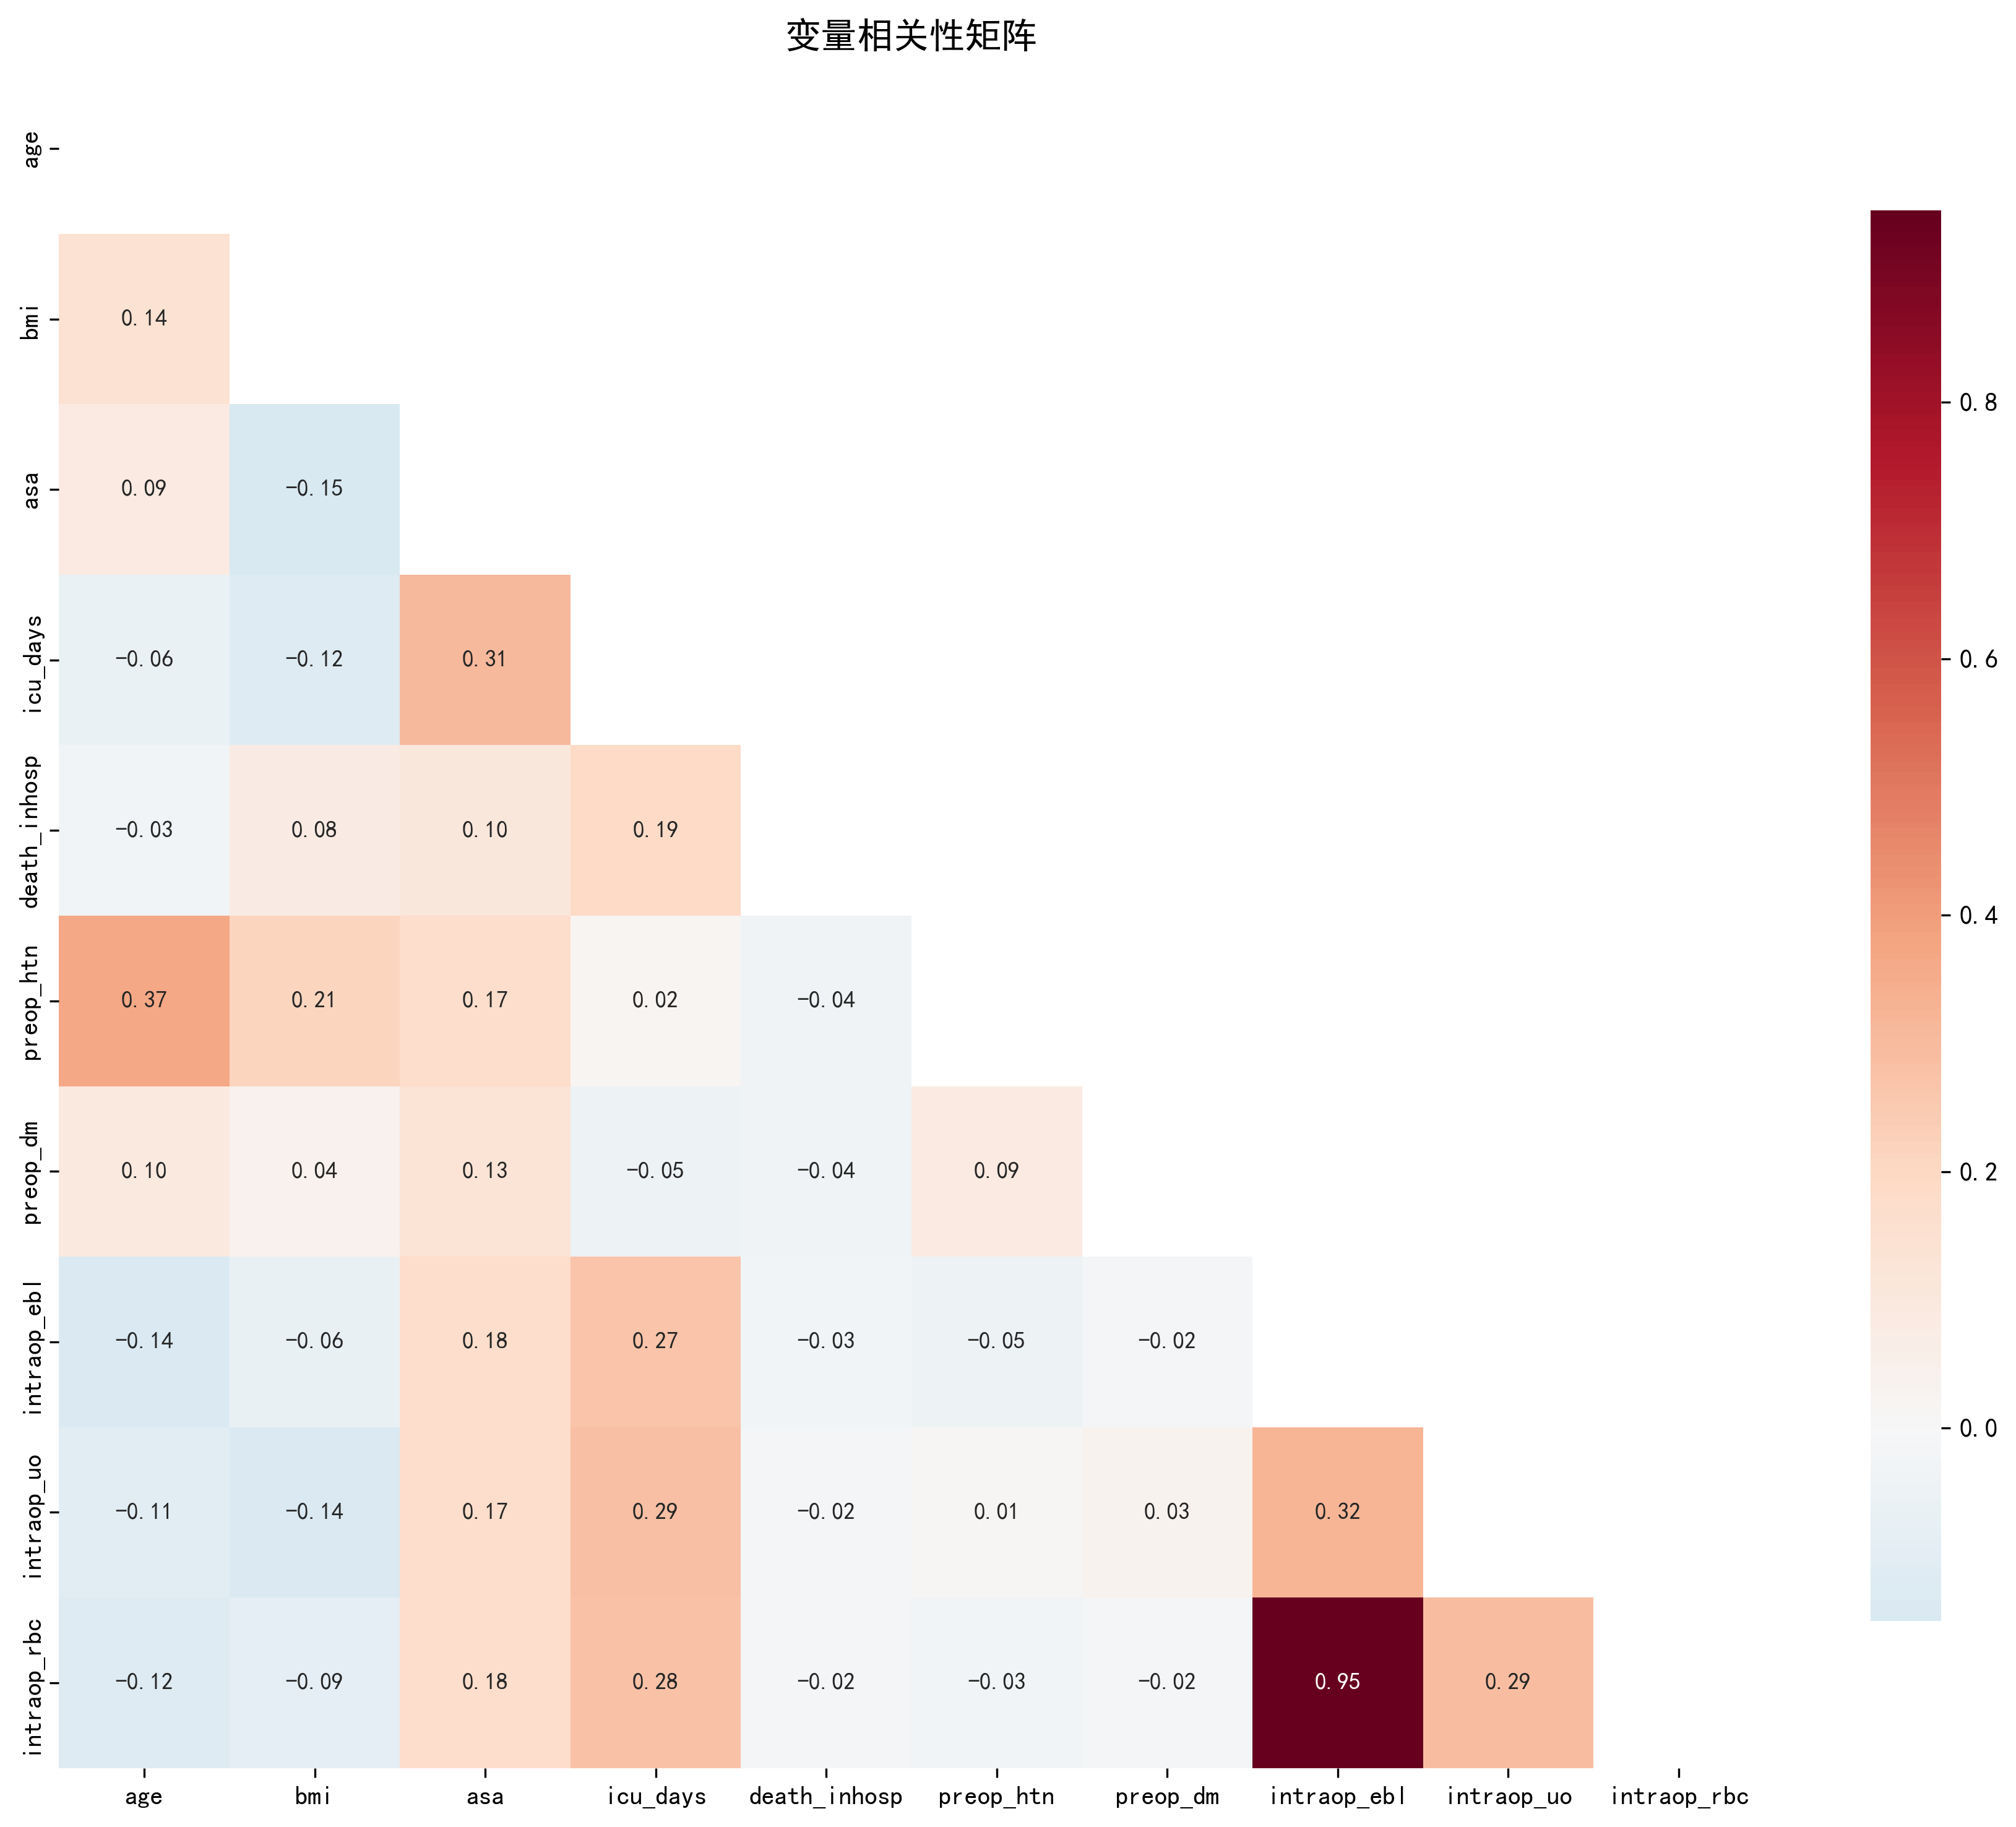
\includegraphics[width=0.8\textwidth]{correlation_heatmap.png}
\caption{Correlation Heatmap of Variables}
\end{figure}

Variables most strongly correlated with mortality:
\begin{enumerate}
    \item \textbf{ICU length of stay} (r = 0.1854)
    \item \textbf{ASA grade} (r = 0.1048)
    \item \textbf{BMI} (r = 0.0788)
\end{enumerate}

\section{Predictive Model Development}

\subsection{Data Preparation}
\begin{itemize}
    \item Feature variables: 10
    \item Target variable: In-hospital mortality
    \item Train/test split: 80\% / 20\%
    \item Class weight adjustment for imbalance
\end{itemize}

\subsection{Model Selection}
\begin{enumerate}
    \item \textbf{Logistic Regression}: High interpretability
    \item \textbf{Random Forest}: Handles non-linear relationships
\end{enumerate}

\section{Model Evaluation and Visualization}

\subsection{Model Performance Comparison}
\begin{figure}[H]
\centering
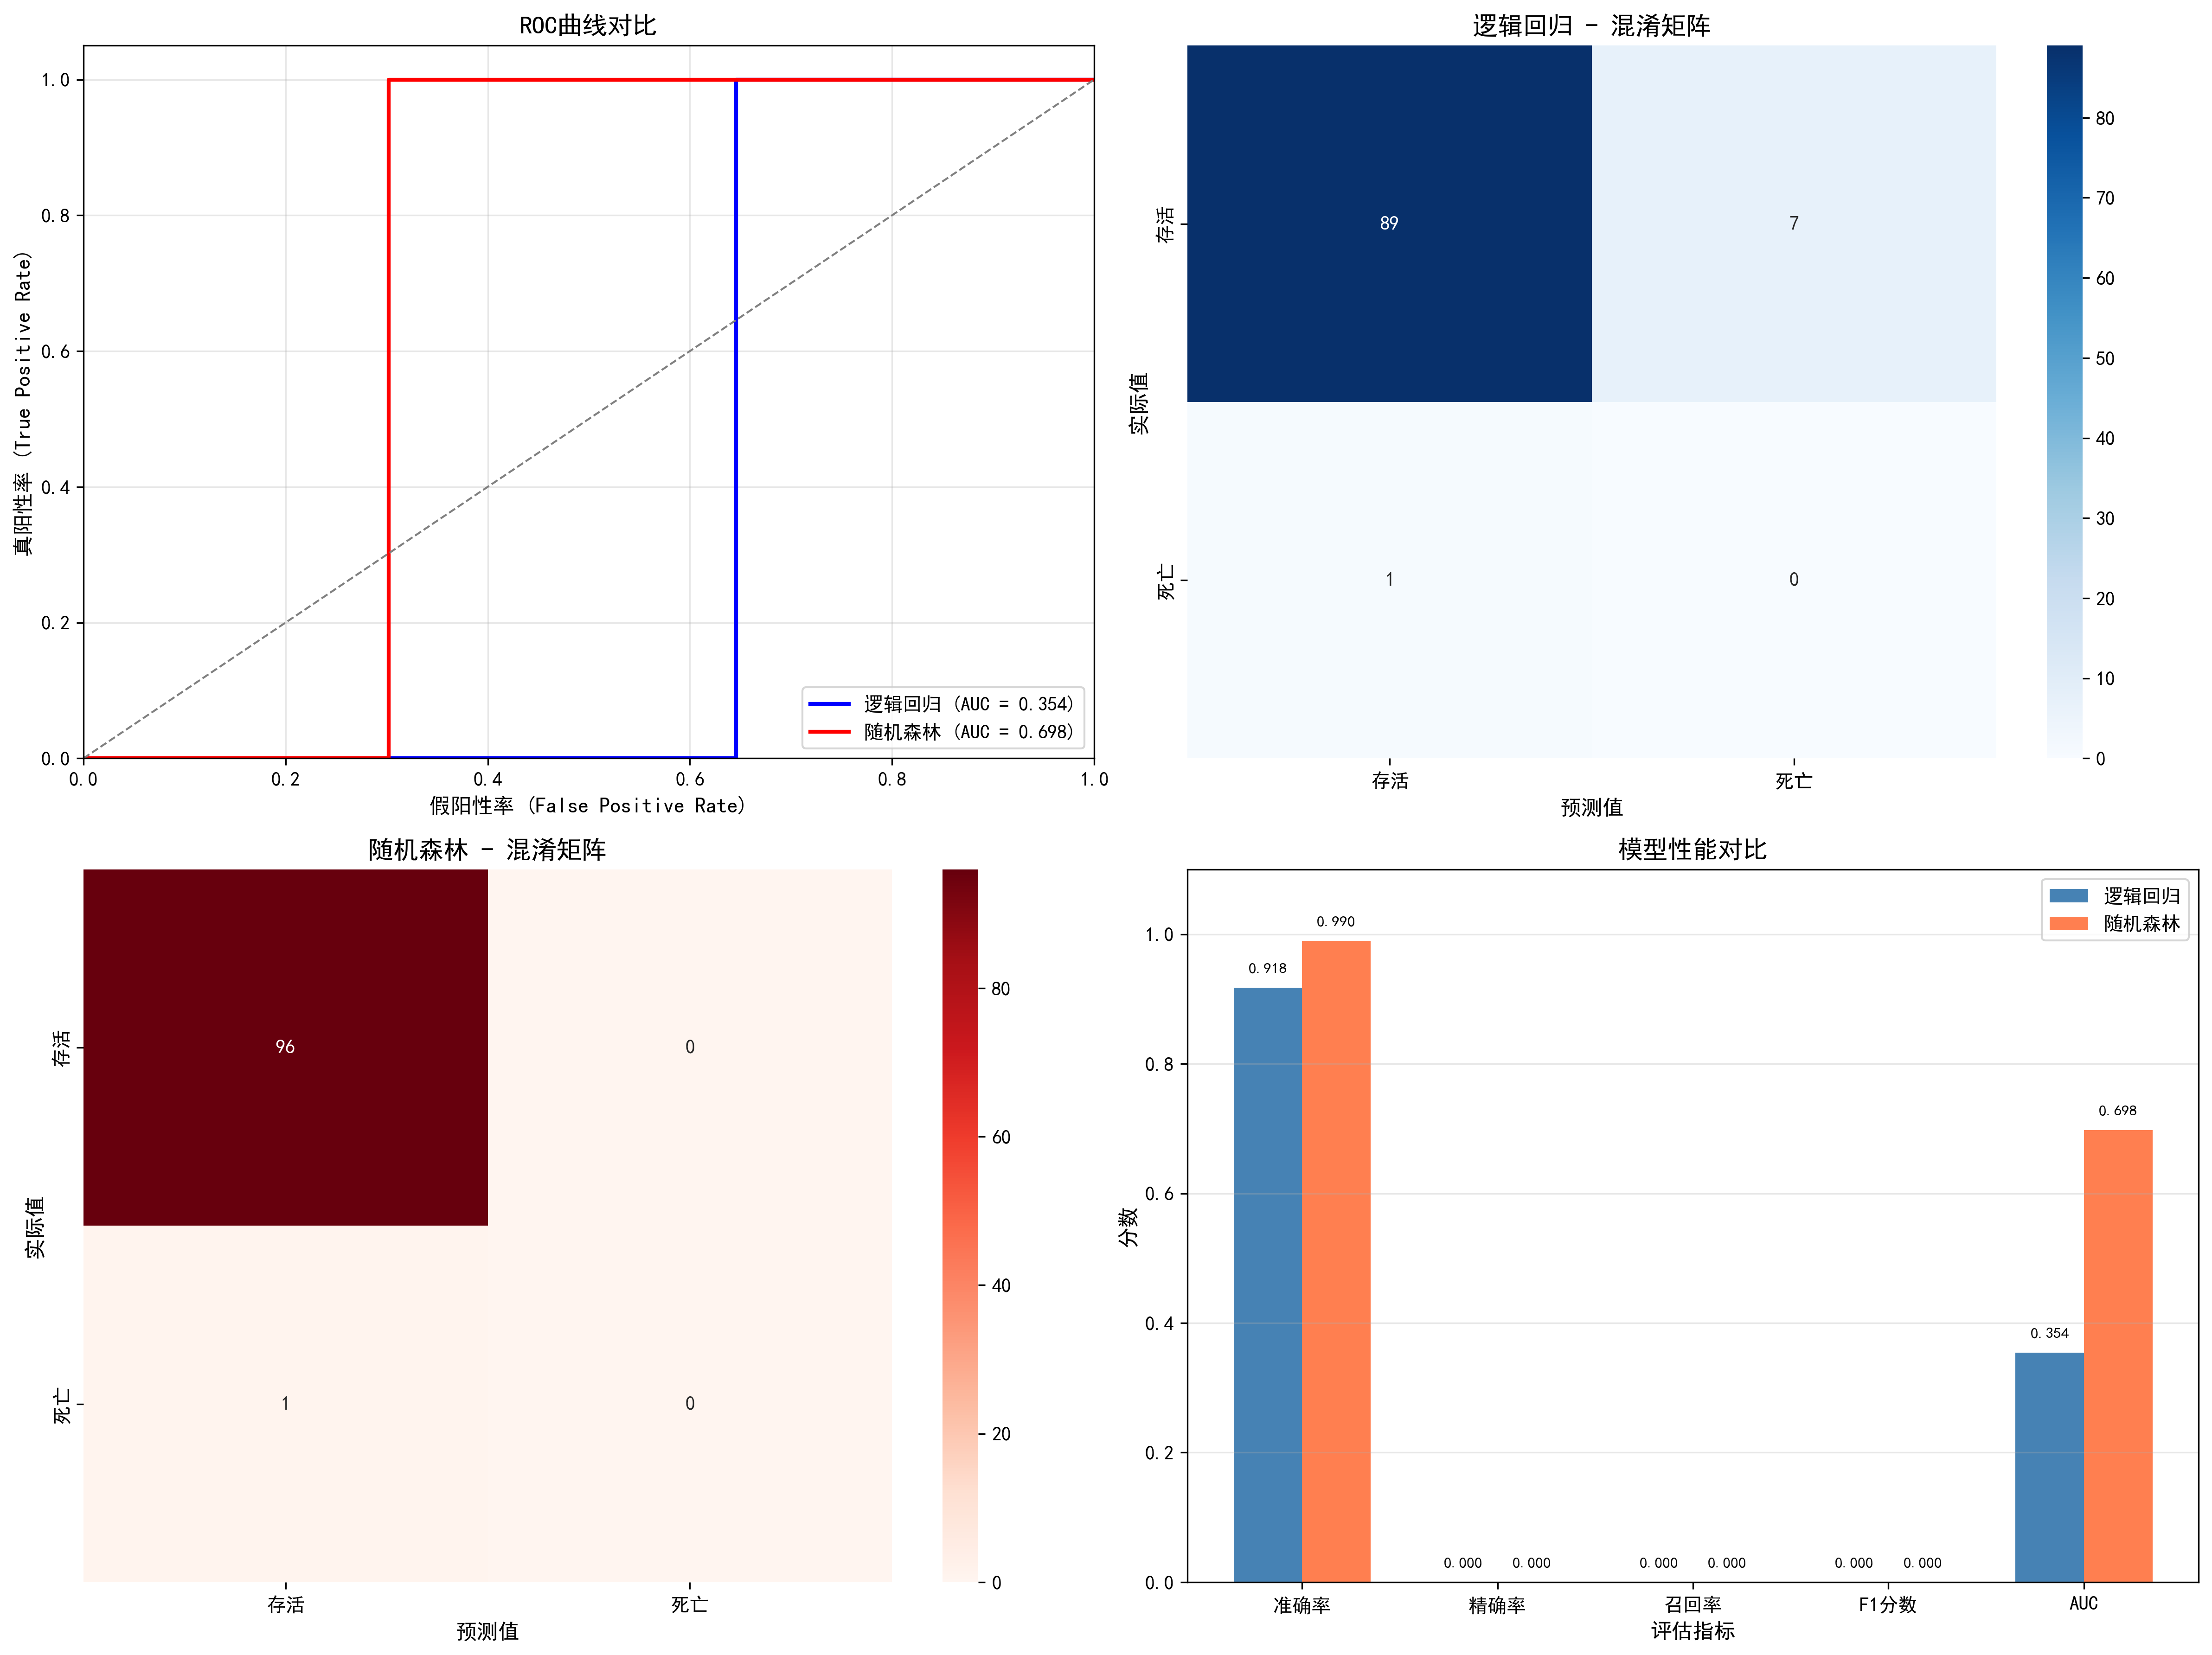
\includegraphics[width=0.9\textwidth]{model_evaluation_comparison.png}
\caption{Model Performance Comparison}
\end{figure}

\begin{table}[H]
\centering
\caption{Model Evaluation Metrics}
\begin{tabular}{lcc}
\toprule
\textbf{Metric} & \textbf{Logistic Regression} & \textbf{Random Forest} \\
\midrule
Accuracy & 0.9175 & \textbf{0.9897} \\
AUC & 0.3542 & \textbf{0.6979} \\
\bottomrule
\end{tabular}
\end{table}

\subsection{Feature Importance Analysis}
\begin{figure}[H]
\centering
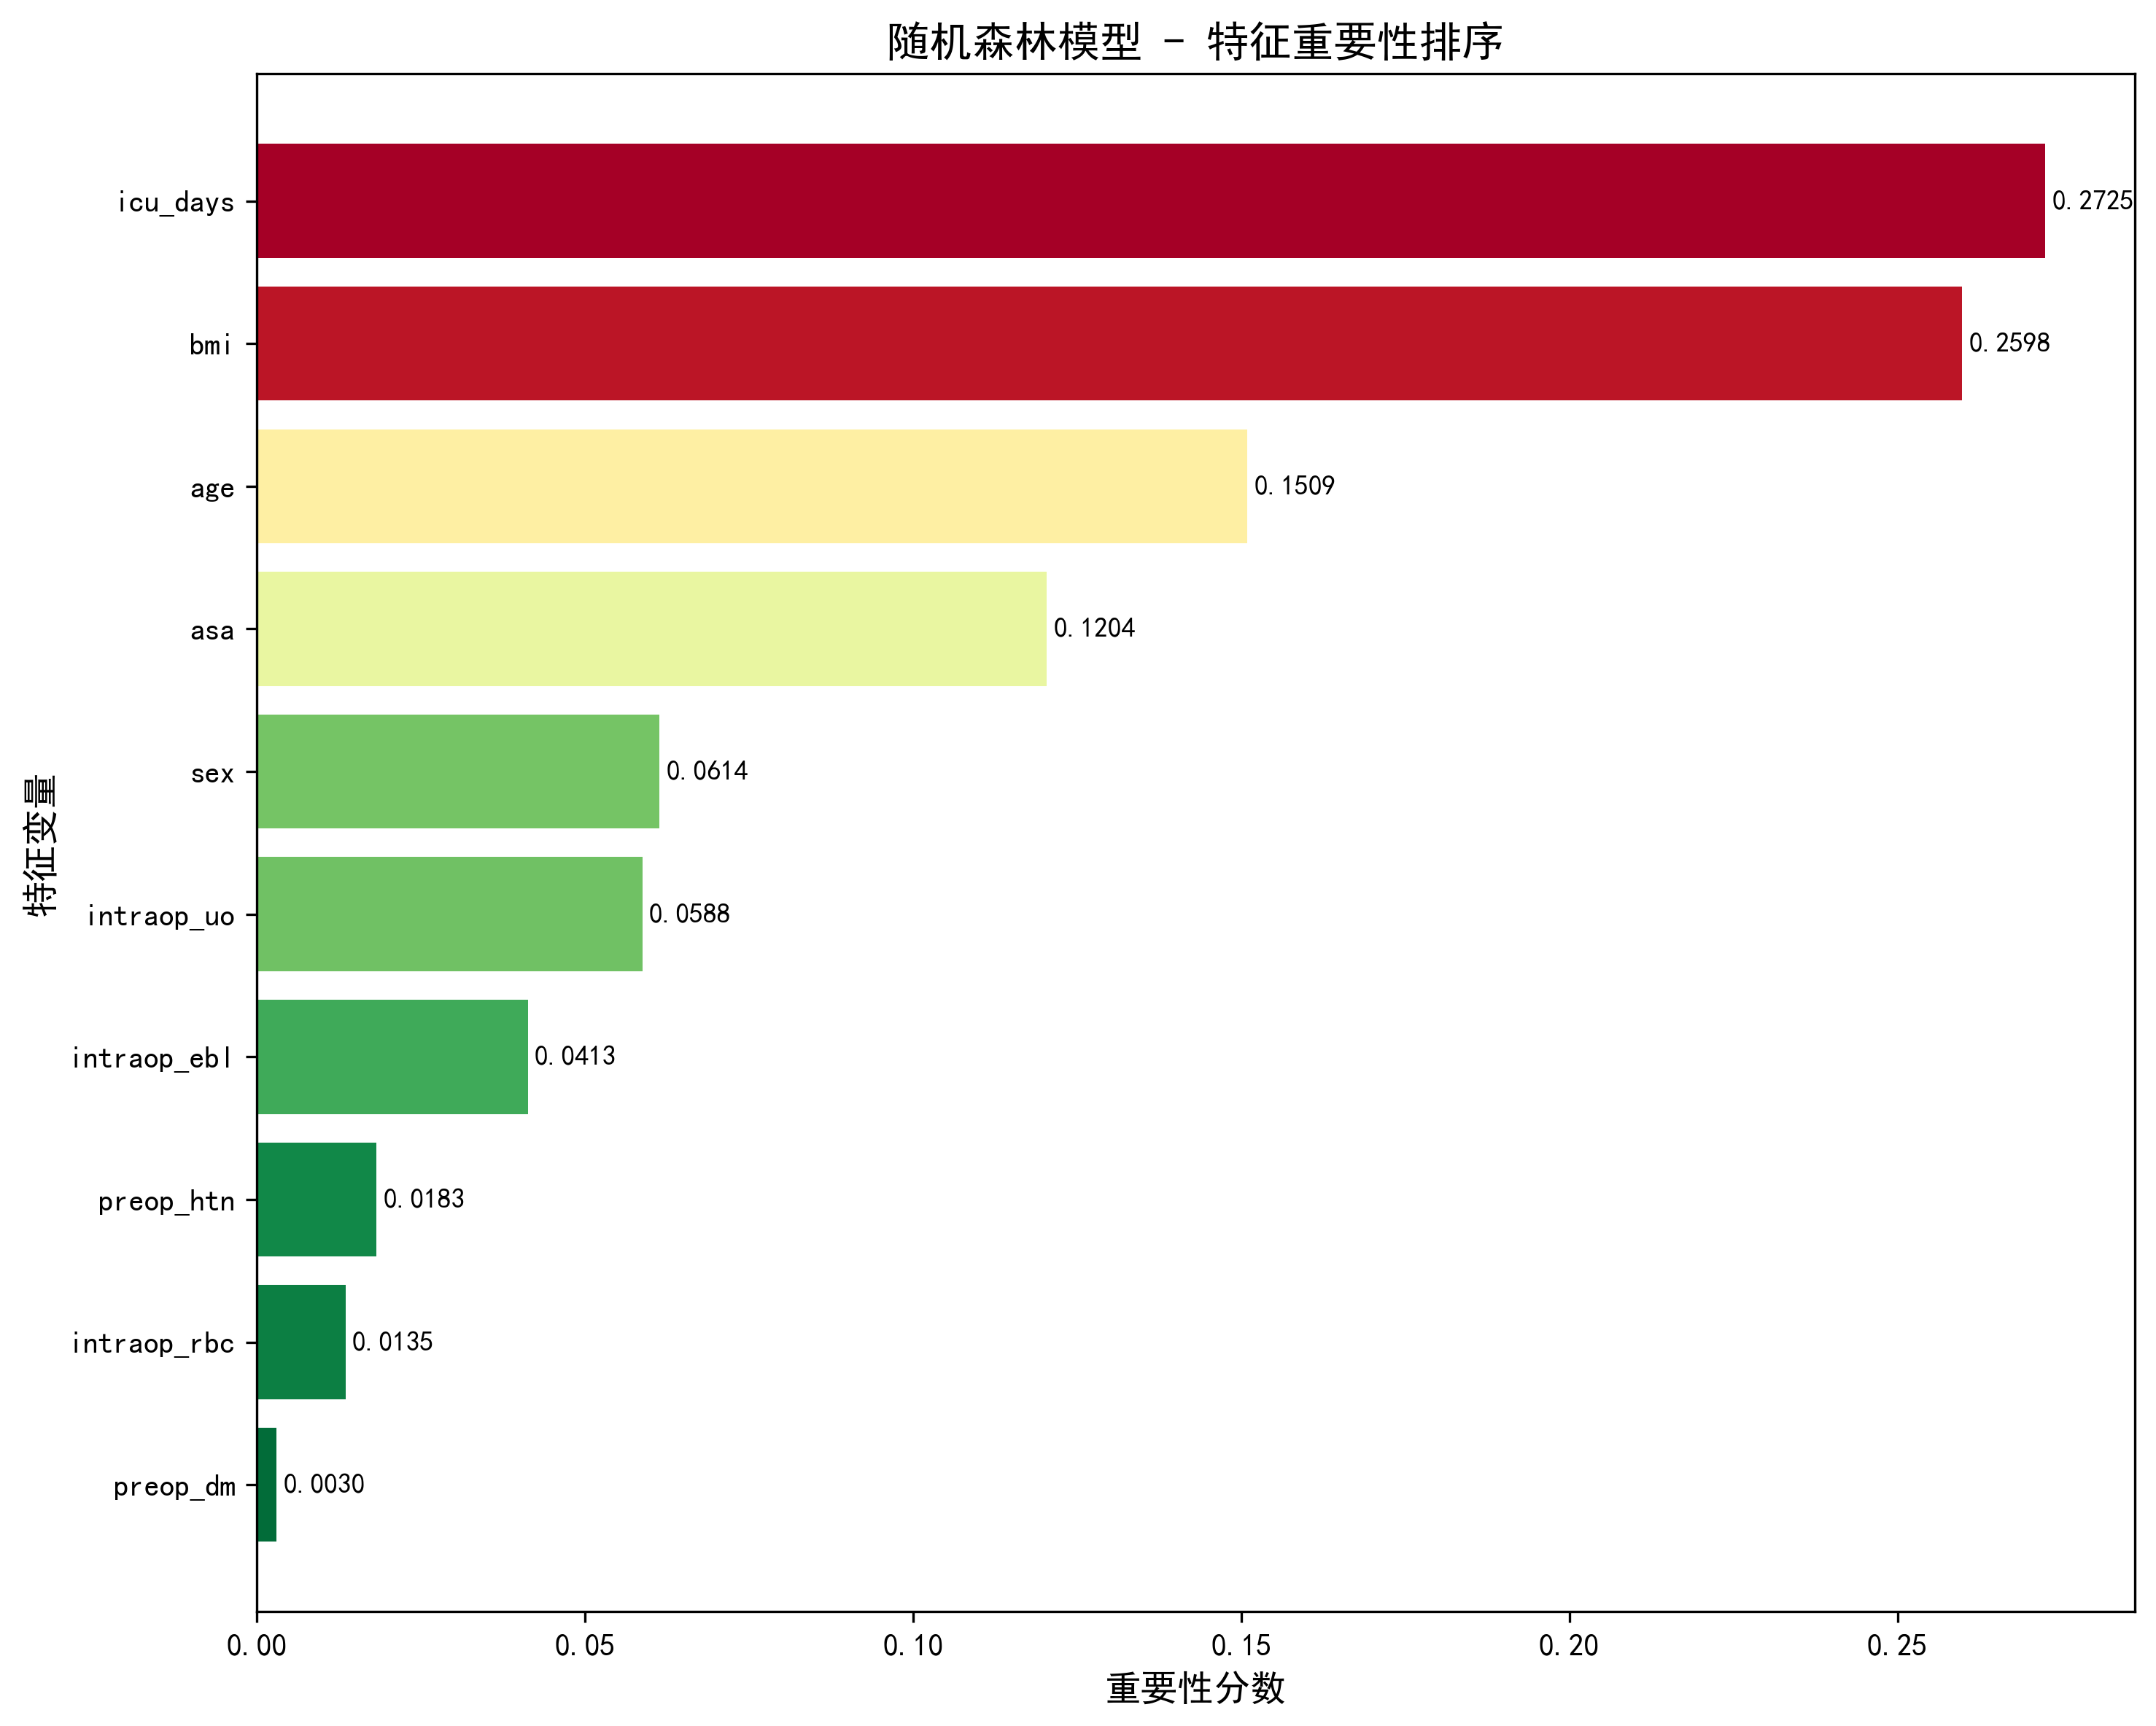
\includegraphics[width=0.7\textwidth]{feature_importance.png}
\caption{Feature Importance Ranking (Random Forest)}
\end{figure}

\begin{table}[H]
\centering
\caption{Top 5 Important Features}
\begin{tabular}{clc}
\toprule
\textbf{Rank} & \textbf{Feature} & \textbf{Importance Score} \\
\midrule
1 & ICU length of stay & 0.2725 \\
2 & BMI & 0.2598 \\
3 & Age & 0.1509 \\
4 & ASA grade & 0.1204 \\
5 & Sex & 0.0614 \\
\bottomrule
\end{tabular}
\end{table}

\section{Conclusions}

\subsection{Main Findings}
\begin{enumerate}
    \item \textbf{ICU length of stay} is the most important predictor of postoperative mortality (p $<$ 0.001)
    \item \textbf{ASA grade} is significantly associated with mortality risk; Grade 3 patients have the highest mortality rate (3.70\%)
    \item \textbf{BMI} and \textbf{age} are also important predictive factors
    \item \textbf{Random forest model} outperforms logistic regression
\end{enumerate}

\subsection{Clinical Implications}
\begin{itemize}
    \item Perioperative attention should focus on patients with \textbf{ASA grade $\geq$ 3}
    \item \textbf{ICU length of stay} is an important prognostic indicator
    \item Enhanced postoperative monitoring is recommended for high-risk patients
\end{itemize}

\subsection{Limitations}
\begin{itemize}
    \item Low mortality rate (only 5 cases) limits model generalizability
    \item Small sample size requires validation with larger cohorts
\end{itemize}

\section*{References}
\begin{enumerate}
    \item Breiman L. Random forests[J]. Machine learning, 2001(10), 45(1): 5-32.
    \item Zou H, Hastie T. Regularization and variable selection via the elastic net[J]. Journal of the Royal Statistical Society. Series B, Statistical methodology, 2005(04), 67(2).
\end{enumerate}

\section*{Appendix}

\textbf{Software Environment}:
\begin{itemize}
    \item Python 3.11
    \item Pandas, Scikit-learn, Matplotlib, Seaborn
\end{itemize}

\textbf{Data Source}: https://physionet.org/content/vitaldb-arrhythmia/1.0.0/metadata.csv

\vfill
\begin{center}
Report Date: April 2026
\end{center}

\end{document}